
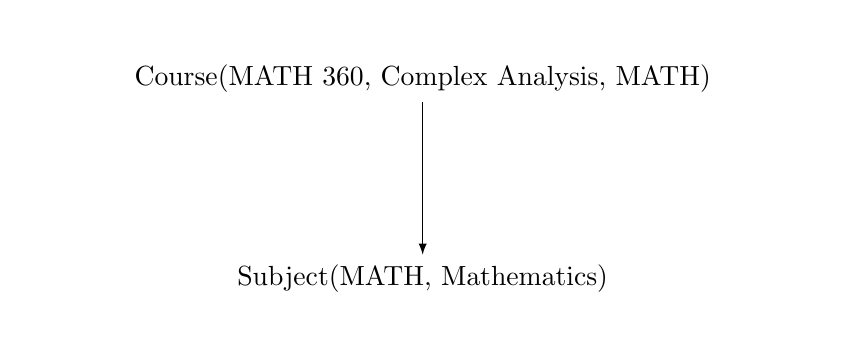
\begin{tikzpicture}[>=latex,line join=bevel,]
%%
\begin{scope}
  \pgfsetstrokecolor{black}
  \definecolor{strokecol}{rgb}{1.0,1.0,1.0};
  \pgfsetstrokecolor{strokecol}
  \definecolor{fillcol}{rgb}{1.0,1.0,1.0};
  \pgfsetfillcolor{fillcol}
  \filldraw (0bp,0bp) -- (0bp,108bp) -- (284bp,108bp) -- (284bp,0bp) -- cycle;
\end{scope}
\begin{scope}
  \pgfsetstrokecolor{black}
  \definecolor{strokecol}{rgb}{1.0,1.0,1.0};
  \pgfsetstrokecolor{strokecol}
  \definecolor{fillcol}{rgb}{1.0,1.0,1.0};
  \pgfsetfillcolor{fillcol}
  \filldraw (0bp,0bp) -- (0bp,108bp) -- (284bp,108bp) -- (284bp,0bp) -- cycle;
\end{scope}
  \node (course) at (142bp,90bp) [draw,draw=none] {Course(MATH 360, Complex Analysis, MATH)};
  \node (subject) at (142bp,18bp) [draw,draw=none] {Subject(MATH, Mathematics)};
  \draw [->] (course) ..controls (142bp,63.983bp) and (142bp,54.712bp)  .. (subject);
%
\end{tikzpicture}
